% !TeX program = xelatex
\documentclass[a4paper,12pt]{report}

\usepackage{hcmus-csc10014-template}

% Tables, lists and figures used in Chapters 1 and 2.
\usepackage{array,longtable,colortbl}
\usepackage{enumitem}
\usepackage{needspace}
\usepackage{placeins}
\definecolor{tablehead}{RGB}{232,240,247}
\setcounter{secnumdepth}{3}
\setcounter{tocdepth}{2}
\setlength{\LTpre}{4pt}
\setlength{\LTpost}{4pt}
\emergencystretch=3em

% Compact headings and float spacing without shrinking body text.
\usepackage{titlesec}
\titlespacing*{\section}{0pt}{12pt plus 2pt minus 2pt}{6pt}
\titlespacing*{\subsection}{0pt}{9pt plus 2pt minus 2pt}{4pt}
\titlespacing*{\subsubsection}{0pt}{7pt plus 1pt minus 1pt}{3pt}
\titleformat{\paragraph}[block]{\normalfont\normalsize\bfseries}{}{0pt}{}
\titlespacing*{\paragraph}{0pt}{6pt}{3pt}
\setlist{topsep=3pt,itemsep=2pt,parsep=0pt,partopsep=0pt}
\setlength{\textfloatsep}{9pt plus 2pt minus 2pt}
\setlength{\floatsep}{8pt plus 2pt minus 2pt}
\setlength{\intextsep}{8pt plus 2pt minus 2pt}
\renewcommand{\topfraction}{0.95}
\renewcommand{\bottomfraction}{0.9}
\renewcommand{\textfraction}{0.08}
\renewcommand{\floatpagefraction}{0.75}
\setcounter{topnumber}{2}
\setcounter{bottomnumber}{2}
\setcounter{totalnumber}{3}
\raggedbottom



% Disable indentation on new paragraphs
% \setlength{\parindent}{0pt}

% Line spacing within the template requirements.
\renewcommand{\baselinestretch}{1.15}

% Optional: graphic path
% \graphicspath{PATH_TO_GRAPHIC_FOLDER}

% Legacy Times fonts are only needed with pdfLaTeX.
% XeLaTeX/LuaLaTeX use the Unicode fonts configured in the template.
\ifPDFTeX
  \usepackage{mathptmx}
\fi

% To use roman section / subsection, uncomment these rows
% \renewcommand{\thesection}{\Roman{section}}
% \renewcommand{\thesubsection}{\thesection.\Roman{subsection}}

% Define course name, report name and report title.
\newcommand{\coursename}{Computational Thinking (CSC10014)}
\newcommand{\reporttitle}{\textit{Midterm} Report}
\newcommand{\reportname}{\textit{WorkspaceAI}}

\newcommand{\studentname}{Hoàng Hải Việt (25127550) \\ Phạm Gia Khiêm (25127378) \\ Đặng Quang Minh (2512417) \\ Hà Lê Bảo Hưng (2512342) \\ Nguyễn Hoàng Minh Duy (25127311) \\ Nguyễn Quang Trường (25127166) \\ Phạm Lâm Viên (25127171)}
\newcommand{\teachername}{Prof. Châu Thành Đức, PhD \\ Assoc. TA. Đỗ Đức Hào, Dr \\ Assoc. TA. Trần Hoàng Quân, M.Sc}

\newcommand{\leftfooter}{\LaTeX\ by \href{https://github.com/trhgquan}{Quan, Tran Hoang}}

% ============ DOCUMENT ============
\begin{document}
	
% Table of Content, List of Figures and List of Tables.
% DO NOT modify this section, unless something is broken.
% \frontmatter
\begin{titlepage}
\newcommand{\HRule}{\rule{\linewidth}{0.5mm}}

\begin{tikzpicture}[remember picture, overlay]
  \draw[line width = 4pt] ($(current page.north west) + (.75in,-.5in)$) rectangle ($(current page.south east) + (-.5in,.5in)$);
\end{tikzpicture}

\centering

\textsc{\Large Vietnam National University Ho Chi Minh City}\\[0.5cm]
\textsc{\Large University of Science}\\[0.5cm]
\textsc{\large Faculty of Information Technology}\\[0.5cm]
% \textsc{Department of Knowledge Engineering}\\[0.5cm]


\includegraphics[scale=.25]{img/hcmus-logo.png}%\\%1cm] 

% \HRule \\[0.4cm]
{ 
\Huge\MakeUppercase{\bfseries{\reporttitle}}\\[0.5cm]
\Large{\bfseries{Project: \reportname}}
}\\[0.5cm]
% \HRule \\[0.5cm]

\textbf{\large Course: \coursename}\\[1.5cm]

\begin{minipage}[t]{0.5\textwidth}
\begin{flushleft} \large
\emph{Students:}\\
\studentname
\end{flushleft}
\end{minipage}
~
\begin{minipage}[t]{0.45\textwidth}
\begin{flushright} \large
\emph{Supervisors:} \\
\teachername
\end{flushright}
\end{minipage}\\[1cm]

\vfill
{\large Ho Chi Minh City, \monthyeardate\today}\\[.5cm]

\end{titlepage}
	

\pagenumbering{roman}
\setcounter{page}{1}

\input{content/guide}

\tableofcontents
\listoffigures
\listoftables
\pagebreak


% \mainmatter
\pagenumbering{arabic}
\setcounter{page}{1}


% Add contents here
% Keep the course Project Brief as reference [1].
\nocite{fit2026projectbrief}
% Synchronized from the Brief Overview tab on 2026-10-29.
% Revised on 2026-10-30 to align with local Ollama architecture and 3-algorithm baseline.

\chapter{Introduction}
\label{chap:introduction}

\begin{quote}\itshape WorkspaceAI \end{quote}

WorkspaceAI is a smart virtual workspace that connects document-based question answering, project-progress reconciliation, and human-approved email reporting. It combines a local large language model (LLM via Ollama) for natural language understanding with explicit Python algorithms for hybrid retrieval, citation verification, progress reconciliation, snapshot hashing, and SMTP email delivery. The following brief outlines the foundational context, objectives, target users, bounded scope, and positioning of the project.

\section{Problem Statement}

Students and project teams often distribute critical information across disparate specifications, spreadsheets, and email drafts. Manually reconciling these fragmented sources to verify requirement completion and prepare progress reports is repetitive, error-prone, and time-consuming. Prior research confirms that individuals frequently struggle to locate and filter relevant source evidence \cite{head2011everyday}, face academic delays from unorganized planning and procrastination \cite{shatz2026procrastination, aeon2021timemanagement}, and incur substantial cognitive overhead managing email updates \cite{mark2016email}. WorkspaceAI addresses this friction through a unified workflow that combines verifiable source-grounded Q\&A, deterministic requirement-task reconciliation, and human-approved email reporting.

\section{Project Objectives}

\Needspace{5\baselineskip}\subsection*{General Objective}

The general objective is to develop a web-based assistant that converts a bounded collection of local project files into verifiable answers, reproducible progress findings, and human-approved academic communication. The application demonstrates a complete computational workflow while keeping language interpretation, deterministic computation, verification, and external action as separate responsibilities.

\Needspace{5\baselineskip}\subsection*{Core Technical Objectives}

\begingroup
\small
\renewcommand{\arraystretch}{1.15}
\setlength{\tabcolsep}{4pt}
\begin{longtable}{|>{\raggedright\arraybackslash}p{\dimexpr 0.23\textwidth-2\tabcolsep-1.5\arrayrulewidth\relax}|>{\raggedright\arraybackslash}p{\dimexpr 0.43\textwidth-2\tabcolsep-1.5\arrayrulewidth\relax}|>{\raggedright\arraybackslash}p{\dimexpr 0.34\textwidth-2\tabcolsep-1.5\arrayrulewidth\relax}|}
\caption{Core technical objectives and empirical verification.}\label{tab:intro-1}\\
\hline
\rowcolor{tablehead}
\textbf{Objective} & \textbf{Implementation target} & \textbf{Evaluation evidence} \\ \hline
\endfirsthead
\multicolumn{3}{l}{\small\itshape Table \thetable\ (continued)}\\
\hline
\rowcolor{tablehead}
\textbf{Objective} & \textbf{Implementation target} & \textbf{Evaluation evidence} \\ \hline
\endhead
\multicolumn{3}{r}{\footnotesize\itshape Continued on next page}\\
\endfoot
\endlastfoot
\textbf{Hybrid retrieval \& citation verification} & Combine BM25Okapi and dense vector embeddings using Reciprocal Rank Fusion (RRF); resolve citations to source locators and check quoted text using exact matching or token-LCS similarity rule. & Measure and report Recall@5 of BM25, vector, and fused retrieval across a defined 30-query test set; reject 100\% of seeded fabricated citations; abstain on unanswerable queries. \\ \hline
\textbf{Deterministic reconciliation engine} & Use pure Python algorithms to compare reviewed requirements $ against task records $; identify uncovered requirements, overdue tasks, and conflicting deadline values against a reference date. & Automated deterministic unit tests for matching rules, missing attributes, date boundaries, and known expected discrepancy findings. \\ \hline
\textbf{Email FSM, SHA-256 digest, \& SMTP gate} & Enforce state transitions \texttt{DRAFT} $\rightarrow$ \texttt{PENDING\_APPROVAL} $\rightarrow$ \texttt{APPROVED}, followed by a separate Send action. Bind approval to canonical SHA-256 payload hash (recipients, subject, body); modifications immediately revoke approval. Submit approved dispatches via Gmail SMTP (STARTTLS, port 587). & Unit tests for payload modification rejection, recipient validation, duplicate dispatch prevention, and logging SENT, FAILED, or DELIVERY\_UNKNOWN outcomes without blind retries. \\ \hline
\end{longtable}
\endgroup

\begin{itemize}[leftmargin=*,itemsep=2pt]
\item \textbf{Grounding limits:} Retrieval evaluation defines explicit evidence units and relevance judgments; unanswerable queries require verified abstention rather than hallucinated answers. Text matching verifies source provenance and locator validity, not absolute semantic entailment.
\item \textbf{Reconciliation semantics:} Stable identifiers and reviewed mappings link requirements to task items. Missing owners, dates, and completion evidence remain explicitly unspecified until resolved by users. Date discrepancies are flagged for human review rather than silently overwritten.
\item \textbf{Controlled external action:} Prompt delimiters mark document text as untrusted data. Email dispatch is strictly decoupled from draft generation: the backend permits at most one transmission per approved SHA-256 digest, and unresolved SMTP delivery outcomes require manual verification.
\end{itemize}

\section{Target End-Users}

\textbf{Individual Students:} Students working independently on coursework or research need to understand assignment specifications, locate evidence across uploaded materials, and organize personal tasks and deadlines. They can ask questions with clickable citations, check personal progress against documented requirements, and review generated status emails before authorizing transmission.

\textbf{Student Project Teams (5–7 Members):} Academic teams need to interpret shared project rubrics, allocate deliverables, assign task ownership, and maintain a synchronized overview of progress. They can compare task boards with source specifications to surface missing deliverables, overdue work, and conflicting deadlines, and prepare human-approved progress reports for team members and advisors.

\textbf{Secondary Users (Instructors and Teaching Assistants):} Teaching staff may inspect student progress records against course milestones and review source-linked evidence. The system facilitates transparency and review; it does not perform automated grading or evaluation.

\section{Project Scope}

\textbf{In scope:} Local PDF (with extractable text layer) and TXT document ingestion, with a maximum limit of 10 active files per workspace and 50 pages per PDF. Document processing preserves file identity, versions, and locators (page numbers for PDF, line ranges for TXT). Tabular CSV/JSON ingestion is treated as an optional stretch goal for task importing.

\textbf{Feature 1 — Evidence-grounded Q\&A:} Users select active sources, ask contextual questions, and inspect supporting passages. The system performs hybrid retrieval (BM25 + vector + RRF), validates citations and quoted text, and abstains when the provided corpus is insufficient.

\textbf{Feature 2 — Document-driven progress management:} Users review proposed requirements and tasks extracted by the local LLM, manage an interactive Kanban board (To Do, In Progress, Done), and execute deterministic Python reconciliation against source requirements to expose missing work, overdue tasks, and conflicting dates.

\textbf{Feature 3 — Context-aware email reporting:} The system drafts progress reports grounded in verified reconciliation findings. Users inspect, edit, and approve an exact snapshot. The backend verifies SHA-256 payload integrity and permits a single dispatch via Gmail SMTP with STARTTLS.

\textbf{Out of scope:} OCR for scanned images or handwriting; autonomous or background email dispatch; runtime web research or Internet scraping; real-time multi-user collaborative editing; automatic grading; and custom LLM model training or fine-tuning. Exploratory artifacts such as mind maps, flashcards, and quizzes are outside this baseline. Google OAuth 2.0 consent, fine-grained role-based access control (RBAC), and email attachments are also excluded.

\textbf{Architectural assumptions:} LLM inference runs locally via Ollama; only outgoing email submission requires network connectivity via authenticated SMTP. Ambiguous requirements and scheduling conflicts require human resolution. Application credentials (SMTP app passwords) reside strictly in backend environment variables and are excluded from prompts, stored documents, and logs.

\section{Related Solutions and Technologies}

\Needspace{5\baselineskip}\subsection*{Qualitative Comparison with Related Solutions}

\begingroup
\small
\renewcommand{\arraystretch}{1.15}
\setlength{\tabcolsep}{4pt}
\begin{longtable}{|>{\raggedright\arraybackslash}p{\dimexpr 0.25\textwidth-2\tabcolsep-1.5\arrayrulewidth\relax}|>{\raggedright\arraybackslash}p{\dimexpr 0.36\textwidth-2\tabcolsep-1.5\arrayrulewidth\relax}|>{\raggedright\arraybackslash}p{\dimexpr 0.39\textwidth-2\tabcolsep-1.5\arrayrulewidth\relax}|}
\caption{Qualitative positioning against documented related solutions.}\label{tab:intro-2}\\
\hline
\rowcolor{tablehead}
\textbf{Solution / category} & \textbf{Documented strengths} & \textbf{WorkspaceAI positioning} \\ \hline
\endfirsthead
\multicolumn{3}{l}{\small\itshape Table \thetable\ (continued)}\\
\hline
\rowcolor{tablehead}
\textbf{Solution / category} & \textbf{Documented strengths} & \textbf{WorkspaceAI positioning} \\ \hline
\endhead
\multicolumn{3}{r}{\footnotesize\itshape Continued on next page}\\
\endfoot
\endlastfoot
\textbf{NotebookLM \cite{googleNotebook}} & Source-grounded Q\&A and citation navigation. & Integrates document Q\&A with deterministic progress reconciliation and human-approved SMTP reporting. \\ \hline
\textbf{Notion AI \cite{notionEnterpriseSearch}} & Workspace search across connected documents. & Applies explicit, inspectable requirement schemas and deterministic Python reconciliation rules. \\ \hline
\textbf{Trello AI Boards \cite{trelloAIBoards}} & Visual Kanban task tracking and automated board creation. & Directly links tasks to source requirement evidence and audits deadline consistency. \\ \hline
\textbf{WorkspaceAI (proposed)} & Local Ollama execution, hybrid RRF retrieval, deterministic reconciliation, and SHA-256 FSM email gating. & Demonstrates an integrated, verifiable academic project workflow with strict human-in-the-loop safeguards. \\ \hline
\end{longtable}
\endgroup

\Needspace{5\baselineskip}\subsection*{Core Technical Foundations}

\begingroup
\small
\renewcommand{\arraystretch}{1.15}
\setlength{\tabcolsep}{4pt}
\begin{longtable}{|>{\raggedright\arraybackslash}p{\dimexpr 0.27\textwidth-2\tabcolsep-1.5\arrayrulewidth\relax}|>{\raggedright\arraybackslash}p{\dimexpr 0.36\textwidth-2\tabcolsep-1.5\arrayrulewidth\relax}|>{\raggedright\arraybackslash}p{\dimexpr 0.37\textwidth-2\tabcolsep-1.5\arrayrulewidth\relax}|}
\caption{Core technical foundations and verification boundaries.}\label{tab:intro-3}\\
\hline
\rowcolor{tablehead}
\textbf{Technology / technique} & \textbf{Proposed role} & \textbf{Verification boundary / limitation} \\ \hline
\endfirsthead
\multicolumn{3}{l}{\small\itshape Table \thetable\ (continued)}\\
\hline
\rowcolor{tablehead}
\textbf{Technology / technique} & \textbf{Proposed role} & \textbf{Verification boundary / limitation} \\ \hline
\endhead
\multicolumn{3}{r}{\footnotesize\itshape Continued on next page}\\
\endfoot
\endlastfoot
\textbf{RAG and source provenance \cite{gao2023citations}} & Grounds LLM responses in retrieved evidence passages. & String and locator matching verifies provenance, not full semantic validity. \\ \hline
\textbf{BM25Okapi + dense embeddings + RRF \cite{cormack2009rrf,brownRankBM25}} & Combines lexical keyword precision with semantic embeddings via Reciprocal Rank Fusion. & RRF scores reflect relative ranking rather than calibrated probabilities; evaluated on frozen test corpora. \\ \hline
\textbf{Deterministic Python reconciliation logic} & Joins requirement and task IDs, computes coverage gaps, and audits deadline discrepancies. & Requires reviewed source mappings and valid date formats; flags ambiguities for user review. \\ \hline
\textbf{Email FSM, SHA-256 digest, \& SMTP \cite{nist2015sha,gmailSMTP}} & State-driven approval workflow, cryptographic payload binding, and authenticated TLS dispatch. & Server acceptance indicates handoff to relay, not guaranteed inbox delivery; requires explicit user initiation. \\ \hline
\end{longtable}
\endgroup

\Needspace{5\baselineskip}\subsection*{Intended Contribution and Project Positioning}

WorkspaceAI integrates established language understanding and software engineering techniques into an inspectable, bounded academic workflow. The fundamental architecture follows a consistent cross-cutting pattern: \textbf{`AI proposes, Python verifies, human decides.''} 
The local LLM assists in understanding unstructured documents and drafting text; deterministic Python algorithms enforce business rules, citation validity, progress reconciliation, and cryptographic snapshot integrity; and human users retain complete decision-making authority over project state and external communication.

% Chapter 2 of the HCMUS Computational Thinking report.

% Fully restructured to align with CSC10014 baseline, local Ollama architecture,

% and the 3-algorithm engineering plan (Hybrid Retrieval, Reconciliation, Email FSM).



\chapter{System Requirements Analysis}

\label{chap:system-requirements}



WorkspaceAI integrates three core functional capabilities: Evidence-Grounded Q\&A (Feature 1), Document-Driven Progress Management (Feature 2), and Context-Aware Email Reporting with Human-in-the-Loop Send (Feature 3). This chapter consolidates the system requirements across computational thinking analysis, functional specifications, measurable quality attributes, and formal Use Case models.



% =========================================================================

% 2.1 FUNCTIONAL REQUIREMENTS & COMPUTATIONAL THINKING ANALYSIS

% =========================================================================

\section{Functional Requirements and Computational Thinking Analysis}

\label{sec:functional-requirements}



The requirements for each subsystem are introduced through five structured analytical criteria: Problem \& Empirical Evidence, Decomposition, Pattern Recognition, Abstraction, and Existing Solutions \& Conceptual Sketch, followed by a consolidated functional requirement inventory. All critical business constraints are directly embedded into the functional statements.



% -------------------------------------------------------------------------

% FEATURE 1

% -------------------------------------------------------------------------

\needspace{3\baselineskip}

\subsection*{Feature 1 - Evidence-Grounded Q\&A}

\label{sec:feature-1}



\paragraph*{Computational Thinking Analysis}

\begin{itemize}[leftmargin=*,itemsep=3pt]

    \item \textbf{Problem \& Empirical Evidence:} Students frequently struggle to locate authoritative passages within lengthy course rubrics and assignment specifications; general-purpose chatbots frequently hallucinate unsupported statements without verifiable citations. Prior information literacy research indicates that university students frequently encounter substantial difficulty in locating, filtering, and cross-referencing relevant source passages within dense academic texts and assignment specifications \cite{head2011everyday}. To measure this in our specific educational context, we plan an empirical pilot study (targeting 15--20 students performing timed requirement lookup tasks over course specifications); findings will be reported in the project's final evaluation.

    \item \textbf{Decomposition:} The end-to-end question-answering workflow is decomposed into discrete processing stages: (1) Document text extraction and chunking with structural locators (page/line), (2) Dual-index construction (lexical inverted index + dense vector index), (3) Hybrid retrieval with Reciprocal Rank Fusion (RRF), (4) Context-constrained prompt assembly, (5) Local LLM answer generation with citation tags, (6) Deterministic citation verification, and (7) UI rendering with clickable source navigation.

    \item \textbf{Pattern Recognition:} Across heterogeneous document inputs, every piece of retrieved text conforms to a uniform schema: $\texttt{Evidence(doc\_id, version, locator, text)}$. User queries follow a standard retrieval-augmented generation pattern: lexical keyword matching and semantic embedding matching are computed independently and merged via reciprocal rank scoring.

    \item \textbf{Abstraction:} Complex document layouts, visual typography, embedded images, and non-text elements are abstracted away. The system models documents purely as ordered, locator-indexed text chunks. Citations are abstracted as discrete references linking claim spans directly to verified source bounding locators.

    \item \textbf{Existing Solutions \& Conceptual Sketch:} Solutions such as NotebookLM \cite{googleNotebook} support cited document Q\&A. WorkspaceAI differentiates itself by executing inference locally via Ollama, enforcing algorithmic citation verification in pure Python, and programmatically abstaining when supporting evidence is insufficient. The conceptual interface consists of a tripartite view: Source Document Library, Conversational Chat Stream, and an Inspectable Evidence Panel.

\end{itemize}



\paragraph*{Functional Requirements}

The functional inventory for Feature 1 contains 5 prioritized requirements.



\begingroup

\small

\setlength{\tabcolsep}{5pt}

\renewcommand{\arraystretch}{1.15}

\begin{longtable}{>{\raggedright\arraybackslash}p{\dimexpr 0.14\textwidth-2\tabcolsep\relax}>{\raggedright\arraybackslash}p{\dimexpr 0.26\textwidth-2\tabcolsep\relax}>{\raggedright\arraybackslash}p{\dimexpr 0.60\textwidth-2\tabcolsep\relax}}

\hline

\rowcolor{tablehead}

\textbf{ID} & \textbf{Function} & \textbf{Condensed Requirement} \\ \hline

\endfirsthead

\hline

\rowcolor{tablehead}

\textbf{ID} & \textbf{Function} & \textbf{Condensed Requirement} \\ \hline

\endhead

\endfoot

\endlastfoot

\textbf{F1-01} & Source Ingestion \& Library & Upload PDF (with extractable text layer) and TXT files; extract text with granular locators (page/line); display explicit errors for unreadable or invalid files; let users select active sources for querying and delete sources (deleted files are excluded from future queries). \\ \hline

\textbf{F1-02} & Contextual Querying & Accept natural-language questions scoped to selected sources; maintain conversation history; resolve multi-turn follow-up queries using immediate dialogue context. \\ \hline

\textbf{F1-03} & Hybrid Retrieval & Retrieve top-$k$ relevant passages using hybrid lexical (BM25Okapi) and dense semantic vector search merged via Reciprocal Rank Fusion (RRF). \\ \hline

\textbf{F1-04} & Grounded Generation \& Abstention & Synthesize answers with inline citation markers strictly from retrieved evidence passages; abstain from answering when retrieved evidence is insufficient. \\ \hline

\textbf{F1-05} & Citation Verification \& Inspection & Deterministically verify each citation (the locator exists and the quoted text matches the source); flag or strip unverified citations; let users open the original passage from a citation. \\ \hline

\end{longtable}

\endgroup



% -------------------------------------------------------------------------

% FEATURE 2

% -------------------------------------------------------------------------

\needspace{3\baselineskip}

\subsection*{Feature 2 - Document-Driven Progress Management}

\label{sec:feature-2}



\paragraph*{Computational Thinking Analysis}

\begin{itemize}[leftmargin=*,itemsep=3pt]

    \item \textbf{Problem \& Empirical Evidence:} In academic team projects, specifications and rubrics exist in static documents, while daily tasks are tracked informally in spreadsheets or chat groups. This disconnect frequently causes missed deliverables, conflicting deadline assumptions, and overdue submissions. Academic procrastination and fragmented project tracking are prevalent challenges in university team projects \cite{shatz2026procrastination}, while empirical meta-analyses establish a strong positive correlation between systematic time management, academic achievement, and reduced project distress \cite{aeon2021timemanagement}. When course rubrics, meeting agreements, and individual task boards are managed in disconnected tools, deliverable omissions and deadline misalignments frequently remain undetected until late in the semester.

    \item \textbf{Decomposition:} The task reconciliation engine is broken down into four distinct computational operations: (1) LLM-assisted requirement and task extraction with source locators, (2) User review and confirmation gate, (3) Kanban task lifecycle state management, (4) Pure Python deterministic reconciliation comparing requirement obligations against task statuses and reference dates.

    \item \textbf{Pattern Recognition:} All project deliverables adhere to uniform structural entities: $\texttt{Requirement}$ and $\texttt{Task}$. The reconciliation algorithm applies three standardized matching rules across all entity pairs: checking requirement coverage ($R \setminus T$), overdue tasks ($T.\text{deadline} < \text{reference\_date}$), and deadline inconsistencies ($R.\text{deadline} \neq T.\text{deadline}$).

    \item \textbf{Abstraction:} Subtasks, discussion threads, complex dependencies, and non-essential metadata are abstracted out. The system models the project using minimal, essential attributes: ID, Title, Description, Deadline, Assignee, Status (To Do, In Progress, Done), and Source Link. All date comparisons are calculated deterministically against an explicit reference date.

    \item \textbf{Existing Solutions \& Conceptual Sketch:} Traditional task tools like Trello \cite{trelloAIBoards} offer visual boards but lack document-grounded verification. WorkspaceAI bridges this gap by automatically linking tasks back to source requirements and performing automated audit reconciliation. The conceptual interface consists of a two-panel layout: an interactive Kanban Board alongside an automated Reconciliation Findings Drawer.

\end{itemize}



\paragraph*{Functional Requirements}

The functional inventory for Feature 2 contains 5 prioritized requirements.



\begingroup

\small

\setlength{\tabcolsep}{5pt}

\renewcommand{\arraystretch}{1.15}

\begin{longtable}{>{\raggedright\arraybackslash}p{\dimexpr 0.14\textwidth-2\tabcolsep\relax}>{\raggedright\arraybackslash}p{\dimexpr 0.26\textwidth-2\tabcolsep\relax}>{\raggedright\arraybackslash}p{\dimexpr 0.60\textwidth-2\tabcolsep\relax}}

\hline

\rowcolor{tablehead}

\textbf{ID} & \textbf{Function} & \textbf{Condensed Requirement} \\ \hline

\endfirsthead

\hline

\rowcolor{tablehead}

\textbf{ID} & \textbf{Function} & \textbf{Condensed Requirement} \\ \hline

\endhead

\endfoot

\endlastfoot

\textbf{F2-01} & Extraction \& Confirmation & Extract candidate requirements and tasks from documents with source links, leaving unsupported fields unassigned or flagged; only items confirmed by the user become official records. \\ \hline

\textbf{F2-02} & Task Management \& Kanban & Create tasks manually, edit and delete tasks (title, description, deadline, assignee, status); display a Kanban board with To Do, In Progress, and Done columns, filterable by status and assignee. \\ \hline

\textbf{F2-03} & Requirement--Task Mapping & Maintain links between requirements and tasks, supporting manual assignment and system suggestions confirmed by the user. \\ \hline

\textbf{F2-04} & Deterministic Reconciliation & Execute pure Python reconciliation against an explicit reference date to identify uncovered requirements, overdue tasks, and conflicting deadlines. \\ \hline

\textbf{F2-05} & Evidence-Backed Findings & Present each finding with its supporting evidence: source requirement excerpt, linked task, and the dates compared. \\ \hline

\end{longtable}

\endgroup



% -------------------------------------------------------------------------

% FEATURE 3

% -------------------------------------------------------------------------

\needspace{3\baselineskip}

\subsection*{Feature 3 - Context-Aware Email Reporting}

\label{sec:feature-3}



\paragraph*{Computational Thinking Analysis}

\begin{itemize}[leftmargin=*,itemsep=3pt]

    \item \textbf{Problem \& Empirical Evidence:} Drafting academic status updates and supervisor progress reports is time-consuming and vulnerable to accidental errors or premature dispatches. Empirical studies of workplace and academic communication demonstrate that email overload, fragmented communication channels, and constant context switching impose significant cognitive friction and anxiety \cite{mark2016email}. While generative language models can accelerate progress drafting, unconstrained autonomous dispatch creates severe risks of transmitting inaccurate milestones, hallucinated commitments, or premature deliverables without human accountability.

    \item \textbf{Decomposition:} The reporting workflow is decomposed into: (1) Structured finding selection and draft synthesis, (2) User review and manual editing, (3) Cryptographic snapshot hashing (SHA-256), (4) Finite State Machine (FSM) approval gate, (5) Authenticated SMTP transmission over STARTTLS, and (6) Delivery status receipt persistence.

    \item \textbf{Pattern Recognition:} Any action causing external side-effects adheres to a strict state pattern: $\texttt{Draft} \rightarrow \texttt{Review} \rightarrow \texttt{Approve Snapshot} \rightarrow \texttt{Execute}$. Across all three features, the core architectural invariant is reinforced: ``AI proposes, Python verifies, human decides.''

    \item \textbf{Abstraction:} Formatting complexities such as rich HTML templates and binary attachments are abstracted away. The email payload is modeled as a canonical tuple: $\texttt{EmailSnapshot(recipients, subject, body)}$. The external email network is abstracted as an SMTP black box returning discrete states: $\texttt{SENT}$, $\texttt{FAILED}$, or $\texttt{DELIVERY\_UNKNOWN}$.

    \item \textbf{Existing Solutions \& Conceptual Sketch:} Standard email clients provide drafts but do not bind approval to specific content versions or verify factual claims. WorkspaceAI provides cryptographic approval binding and factual grounding from reconciliation findings. The conceptual interface features an Email Composer with a live Snapshot Approval Banner and Transmission Audit Log.

\end{itemize}



\paragraph*{Functional Requirements}

The functional inventory for Feature 3 contains 5 prioritized requirements.



\begingroup

\small

\setlength{\tabcolsep}{5pt}

\renewcommand{\arraystretch}{1.15}

\begin{longtable}{>{\raggedright\arraybackslash}p{\dimexpr 0.14\textwidth-2\tabcolsep\relax}>{\raggedright\arraybackslash}p{\dimexpr 0.26\textwidth-2\tabcolsep\relax}>{\raggedright\arraybackslash}p{\dimexpr 0.60\textwidth-2\tabcolsep\relax}}

\hline

\rowcolor{tablehead}

\textbf{ID} & \textbf{Function} & \textbf{Condensed Requirement} \\ \hline

\endfirsthead

\hline

\rowcolor{tablehead}

\textbf{ID} & \textbf{Function} & \textbf{Condensed Requirement} \\ \hline

\endhead

\endfoot

\endlastfoot

\textbf{F3-01} & Grounded Draft Synthesis & Generate email drafts (recipients, subject, body, citations) from verified reconciliation findings or selected evidence; omit or flag claims lacking verified provenance. \\ \hline

\textbf{F3-02} & Manual Composition \& Validation & Allow manual composition and editing of drafts without AI; validate recipient address format and reject dispatch for invalid addresses. \\ \hline

\textbf{F3-03} & Snapshot Approval \& Invalidation & Provide draft preview and explicit approval; store the SHA-256 hash of the approved payload (recipients, subject, body); revoke approval automatically when any of these fields change. \\ \hline

\textbf{F3-04} & Controlled Dispatch via SMTP & Require a separate, explicit Send action; send only when the state is APPROVED and the hash matches, at most once per snapshot; transmit via Gmail SMTP with STARTTLS (port 587) and record SENT, FAILED, or DELIVERY\_UNKNOWN without automatic retries. \\ \hline

\textbf{F3-05} & Audit History & Keep a history of draft versions, approval times, snapshot hashes, and transmission outcomes. \\ \hline

\end{longtable}

\endgroup



% =========================================================================

% 2.2 NON-FUNCTIONAL REQUIREMENTS

% =========================================================================

\needspace{3\baselineskip}

\section{Non-functional Requirements}

\label{sec:non-functional-requirements}



To ensure empirical verifiability under realistic student computing environments, non-functional requirements are consolidated into 7 measurable quality attributes. Unrealistic enterprise metrics (such as 99.99\% high availability clusters or complex disaster recovery RTOs) are replaced with concrete, reproducible evaluation procedures.



\begingroup

\small

\setlength{\tabcolsep}{5pt}

\renewcommand{\arraystretch}{1.2}

\begin{longtable}{>{\raggedright\arraybackslash}p{\dimexpr 0.12\textwidth-2\tabcolsep\relax}>{\raggedright\arraybackslash}p{\dimexpr 0.22\textwidth-2\tabcolsep\relax}>{\raggedright\arraybackslash}p{\dimexpr 0.66\textwidth-2\tabcolsep\relax}}

\hline

\rowcolor{tablehead}

\textbf{ID} & \textbf{Quality Area} & \textbf{Measurable Target and Verification Method} \\ \hline

\endfirsthead

\hline

\rowcolor{tablehead}

\textbf{ID} & \textbf{Quality Area} & \textbf{Measurable Target and Verification Method} \\ \hline

\endhead

\endfoot

\endlastfoot

\textbf{NFR-01} & Performance & Standard UI interactions (Kanban updates, filtering, tab navigation) respond within $\le$ 3 s. Local LLM generation (Q\&A, draft synthesis) targets $\le$ 60 s on the demonstration testbed (Ollama local inference) with real-time streaming progress indication. Evaluated across 10 benchmark executions reporting mean and maximum latency. \\ \hline

\textbf{NFR-02} & Retrieval Accuracy & Evaluated on a curated 30-query academic test set (including $\approx$ 5 unanswerable queries). The system must report Recall@5 across BM25, dense vector, and RRF retrieval; reject 100\% of seeded fabricated citations (5–10 adversarial test cases); and correctly abstain on unanswerable queries. \\ \hline

\textbf{NFR-03} & Security \& Privacy & Local-first processing ensures source documents and conversational prompts never leave the local environment. SMTP credentials reside exclusively in backend environment configurations (\texttt{.env}) and are excluded from prompts and logs. Document text is encapsulated within untrusted data delimiters to mitigate prompt injection. \\ \hline

\textbf{NFR-04} & Integrity \& Reliability & Deterministic verification for the email FSM and SHA-256 digest: any payload tampering halts transmission; duplicate dispatches are blocked. Failed storage or transmission operations never report false success. LLM provider timeouts or malformed JSON outputs trigger at most 1–2 automated retries before returning an explicit, graceful error. \\ \hline

\textbf{NFR-05} & Usability & Clear visual feedback during background computations; status distinctions are conveyed through iconography and text rather than color alone. Usability is verified through pilot testing with 3–5 representative students, requiring $\ge$ 4/5 participants to complete primary workflows without external assistance. \\ \hline

\textbf{NFR-06} & Compatibility & Verified on latest stable desktop releases of Google Chrome, Microsoft Edge, and Mozilla Firefox. Supports documents in English and Vietnamese, with documented language capability boundaries of the selected local LLM model. \\ \hline

\textbf{NFR-07} & Maintainability & Clean separation of concerns across ingestion, retrieval, reconciliation, and email delivery modules. Model parameters, Ollama endpoints, and ingestion thresholds are externalized in configuration files. Core Python algorithms are covered by automated unit test suites with instructions provided in the project README. \\ \hline

\end{longtable}

\endgroup



% =========================================================================

% 2.3 USE CASE MODELING

% =========================================================================

\needspace{3\baselineskip}

\section{Use Case Modeling}

\label{sec:use-case-modeling}



The operational boundaries and user interactions of WorkspaceAI are formally modeled using a unified Use Case diagram, nine comprehensive specifications, and an end-to-end requirement traceability matrix. All use cases assume an authenticated \textbf{Workspace Member} operating within an authorized workspace context.



\subsection{Overall Use Case Diagram}

\label{subsec:overall-use-case-diagram}



The overall system interactions are structured around a single primary actor (\textbf{Workspace Member}) and a single external supporting actor (\textbf{SMTP Server}). Local LLM inference (via Ollama) operates within the internal system boundary.



\begin{figure}[!htbp]

\centering

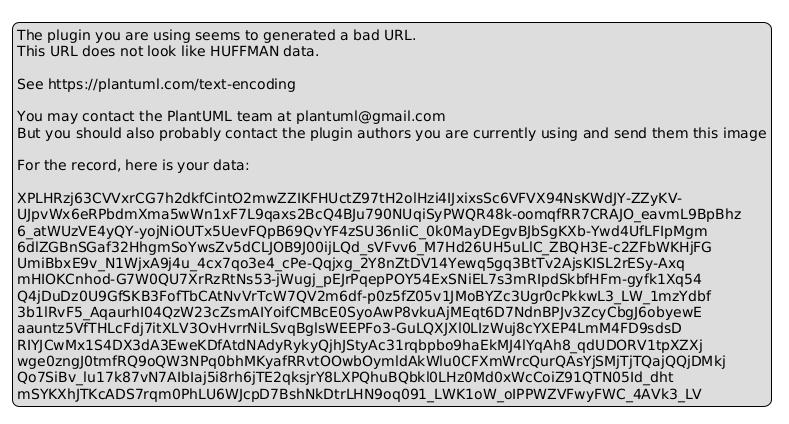
\includegraphics[width=0.88\linewidth,keepaspectratio]{img/chapter2/overall-use-case.png}

\caption{Overall Use Case Diagram for WorkspaceAI.}

\label{fig:overall-use-case}

\end{figure}



The diagram embodies three fundamental architectural constraints:

\begin{enumerate}[leftmargin=*,itemsep=1pt]

    \item All user interactions require an active workspace session.

    \item Source documents ingested in UC-01 serve as shared preconditions for requirement extraction (UC-04) and contextual email drafting (UC-07); reconciliation findings from UC-06 feed directly into status reporting (UC-07).

    \item Citation verification is encapsulated as a reusable $\ll\text{include}\gg$ dependency utilized by both Q\&A generation (UC-02) and email drafting (UC-07), illustrating the consistent verification pattern.

\end{enumerate}



\needspace{3\baselineskip}

\subsection{Use Case Specifications}

\label{subsec:use-case-specifications}



The nine core use cases are formally specified below using a standardized specification structure.



% --- UC-01 ---

\paragraph*{UC-01: Upload and Manage Sources}

\begingroup

\small

\setlength{\tabcolsep}{5pt}

\renewcommand{\arraystretch}{1.1}

\begin{longtable}{>{\raggedright\arraybackslash}p{\dimexpr 0.22\textwidth-2\tabcolsep\relax}>{\raggedright\arraybackslash}p{\dimexpr 0.78\textwidth-2\tabcolsep\relax}}

\hline

\rowcolor{tablehead}

\textbf{Attribute} & \textbf{Specification Details} \\ \hline

\endfirsthead

\hline

\rowcolor{tablehead}

\textbf{Attribute} & \textbf{Specification Details} \\ \hline

\endhead

\endfoot

\endlastfoot

\textbf{ID / Name} & UC-01: Upload and Manage Sources \\ \hline

\textbf{Actor} & Workspace Member \\ \hline

\textbf{Related FR} & F1-01 \\ \hline

\textbf{Preconditions} & User is authenticated and has write access to the active workspace. \\ \hline

\textbf{Trigger} & User uploads a file or accesses the document library panel. \\ \hline

\textbf{Basic Flow} & \begin{enumerate}[nosep,leftmargin=*,label=\arabic*.]

    \item User selects one or more PDF/TXT files and initiates upload.

    \item System verifies file format and size limits, then extracts text and records locator metadata (page numbers, line offsets).

    \item System generates dual indices (BM25 lexical and dense vector representations).

    \item System updates the Document Library, displaying the source as Ready for querying.

    \item User selects or deselects sources to define the active retrieval scope.

\end{enumerate} \\ \hline

\textbf{Alternate Flow} & \begin{enumerate}[nosep,leftmargin=*,label=\arabic*.]

    \item A1 - Delete source: User deletes an existing source; the system purges its index and excludes it from future queries.

\end{enumerate} \\ \hline

\textbf{Exception Flow} & \begin{enumerate}[nosep,leftmargin=*,label=\arabic*.]

    \item E1 - Unreadable or invalid file: System rejects the file, marks status as Failed, and displays an actionable error message without crashing.

\end{enumerate} \\ \hline

\textbf{Postconditions} & Success: Extracted source is indexed and available in the library. Failure: Invalid file is rejected; workspace state remains unchanged. \\ \hline

\end{longtable}

\endgroup



% --- UC-02 ---

\needspace{3\baselineskip}

\paragraph*{UC-02: Ask Source-Grounded Question}

\begingroup

\small

\setlength{\tabcolsep}{5pt}

\renewcommand{\arraystretch}{1.1}

\begin{longtable}{>{\raggedright\arraybackslash}p{\dimexpr 0.22\textwidth-2\tabcolsep\relax}>{\raggedright\arraybackslash}p{\dimexpr 0.78\textwidth-2\tabcolsep\relax}}

\hline

\rowcolor{tablehead}

\textbf{Attribute} & \textbf{Specification Details} \\ \hline

\endfirsthead

\hline

\rowcolor{tablehead}

\textbf{Attribute} & \textbf{Specification Details} \\ \hline

\endhead

\endfoot

\endlastfoot

\textbf{ID / Name} & UC-02: Ask Source-Grounded Question \\ \hline

\textbf{Actor} & Workspace Member \\ \hline

\textbf{Related FR} & F1-02, F1-03, F1-04, F1-05 \\ \hline

\textbf{Preconditions} & At least one usable source is selected in the active workspace. \\ \hline

\textbf{Trigger} & User enters a natural language query in the chat input box. \\ \hline

\textbf{Basic Flow} & \begin{enumerate}[nosep,leftmargin=*,label=\arabic*.]

    \item User submits a query relating to selected documents.

    \item System executes hybrid retrieval (BM25 + vector search) and ranks passages using RRF.

    \item System verifies that top passages satisfy the relevance threshold.

    \item Local LLM generates an evidence-grounded response with inline citation markers.

    \item System executes $\ll\text{include}\gg$ Verify Citations to validate citation locators and quoted snippets.

    \item System renders the verified answer and clickable citation badges in the chat view.

\end{enumerate} \\ \hline

\textbf{Alternate Flow} & \begin{enumerate}[nosep,leftmargin=*,label=\arabic*.]

    \item A1 - Insufficient evidence: Retrieved passages do not meet the relevance threshold; system abstains and advises the user that the selected sources lack the answer.

\end{enumerate} \\ \hline

\textbf{Exception Flow} & \begin{enumerate}[nosep,leftmargin=*,label=\arabic*.]

    \item E1 - Local LLM offline or timeout: System detects Ollama failure, notifies the user, and preserves the conversation state for retry.

\end{enumerate} \\ \hline

\textbf{Postconditions} & Success: Grounded answer with verified citations is appended to the chat session. Failure: User is notified; no fabricated answer is stored. \\ \hline

\end{longtable}

\endgroup



% --- UC-03 ---

\needspace{3\baselineskip}

\paragraph*{UC-03: Inspect Citation}

\begingroup

\small

\setlength{\tabcolsep}{5pt}

\renewcommand{\arraystretch}{1.1}

\begin{longtable}{>{\raggedright\arraybackslash}p{\dimexpr 0.22\textwidth-2\tabcolsep\relax}>{\raggedright\arraybackslash}p{\dimexpr 0.78\textwidth-2\tabcolsep\relax}}

\hline

\rowcolor{tablehead}

\textbf{Attribute} & \textbf{Specification Details} \\ \hline

\endfirsthead

\hline

\rowcolor{tablehead}

\textbf{Attribute} & \textbf{Specification Details} \\ \hline

\endhead

\endfoot

\endlastfoot

\textbf{ID / Name} & UC-03: Inspect Citation \\ \hline

\textbf{Actor} & Workspace Member \\ \hline

\textbf{Related FR} & F1-05, F3-01 \\ \hline

\textbf{Preconditions} & An answer or email draft containing citations is displayed. \\ \hline

\textbf{Trigger} & User clicks on an inline citation badge. \\ \hline

\textbf{Basic Flow} & \begin{enumerate}[nosep,leftmargin=*,label=\arabic*.]

    \item User clicks a citation badge in an answer or email preview.

    \item System resolves the document ID, version, and locator coordinates (page/line).

    \item System opens the Evidence Viewer side panel and highlights the exact cited passage in context.

    \item User reviews the supporting text and closes the panel to return to the active workflow.

\end{enumerate} \\ \hline

\textbf{Alternate Flow} & \begin{enumerate}[nosep,leftmargin=*,label=\arabic*.]

    \item A1 - Multiple supporting passages: System lists all cited fragments, allowing the user to cycle through them.

\end{enumerate} \\ \hline

\textbf{Exception Flow} & \begin{enumerate}[nosep,leftmargin=*,label=\arabic*.]

    \item E1 - Source file deleted: System displays a notice that the referenced source has been removed, displaying saved text snippet only.

\end{enumerate} \\ \hline

\textbf{Postconditions} & Success: Exact cited passage is displayed with contextual locator metadata. \\ \hline

\end{longtable}

\endgroup



% --- UC-04 ---

\needspace{3\baselineskip}

\paragraph*{UC-04: Extract and Review Requirements/Tasks}

\begingroup

\small

\setlength{\tabcolsep}{5pt}

\renewcommand{\arraystretch}{1.1}

\begin{longtable}{>{\raggedright\arraybackslash}p{\dimexpr 0.22\textwidth-2\tabcolsep\relax}>{\raggedright\arraybackslash}p{\dimexpr 0.78\textwidth-2\tabcolsep\relax}}

\hline

\rowcolor{tablehead}

\textbf{Attribute} & \textbf{Specification Details} \\ \hline

\endfirsthead

\hline

\rowcolor{tablehead}

\textbf{Attribute} & \textbf{Specification Details} \\ \hline

\endhead

\endfoot

\endlastfoot

\textbf{ID / Name} & UC-04: Extract and Review Requirements/Tasks \\ \hline

\textbf{Actor} & Workspace Member \\ \hline

\textbf{Related FR} & F2-01 \\ \hline

\textbf{Preconditions} & A project specification or rubric document has been uploaded. \\ \hline

\textbf{Trigger} & User selects ``Extract Tasks from Document'' on the Task Board. \\ \hline

\textbf{Basic Flow} & \begin{enumerate}[nosep,leftmargin=*,label=\arabic*.]

    \item User selects a target document and initiates extraction.

    \item Local LLM analyzes the text and produces structured requirement and task candidates.

    \item System populates the Review Drawer with proposed items (title, description, deadline, source link).

    \item User edits fields, discards invalid suggestions, or adds missing entries.

    \item User clicks ``Confirm and Save''; system persists approved items to the workspace database.

\end{enumerate} \\ \hline

\textbf{Alternate Flow} & \begin{enumerate}[nosep,leftmargin=*,label=\arabic*.]

    \item A1 - Missing details: Unsupported deadlines or assignees are flagged as ``unspecified'' for manual input.

\end{enumerate} \\ \hline

\textbf{Exception Flow} & \begin{enumerate}[nosep,leftmargin=*,label=\arabic*.]

    \item E1 - Extraction schema validation failure: System detects invalid LLM JSON output, retries once, and falls back to manual entry prompt.

\end{enumerate} \\ \hline

\textbf{Postconditions} & Success: Only user-confirmed items are persisted as official requirements and tasks. Failure: Proposals discarded; database unchanged. \\ \hline

\end{longtable}

\endgroup



% --- UC-05 ---

\needspace{3\baselineskip}

\paragraph*{UC-05: Manage Tasks on Kanban Board}

\begingroup

\small

\setlength{\tabcolsep}{5pt}

\renewcommand{\arraystretch}{1.1}

\begin{longtable}{>{\raggedright\arraybackslash}p{\dimexpr 0.22\textwidth-2\tabcolsep\relax}>{\raggedright\arraybackslash}p{\dimexpr 0.78\textwidth-2\tabcolsep\relax}}

\hline

\rowcolor{tablehead}

\textbf{Attribute} & \textbf{Specification Details} \\ \hline

\endfirsthead

\hline

\rowcolor{tablehead}

\textbf{Attribute} & \textbf{Specification Details} \\ \hline

\endhead

\endfoot

\endlastfoot

\textbf{ID / Name} & UC-05: Manage Tasks on Kanban Board \\ \hline

\textbf{Actor} & Workspace Member \\ \hline

\textbf{Related FR} & F2-02 \\ \hline

\textbf{Preconditions} & User is inside an active workspace. \\ \hline

\textbf{Trigger} & User interacts with the Kanban Board view. \\ \hline

\textbf{Basic Flow} & \begin{enumerate}[nosep,leftmargin=*,label=\arabic*.]

    \item User accesses the Kanban Board, viewing tasks grouped under To Do, In Progress, and Done.

    \item User creates a new task manually, or edits existing task attributes (title, deadline, assignee, status).

    \item User drags a task card between status columns to update completion progress.

    \item System validates changes and persists them to the local database.

    \item Board refreshes immediately, maintaining state across browser reloads.

\end{enumerate} \\ \hline

\textbf{Alternate Flow} & \begin{enumerate}[nosep,leftmargin=*,label=\arabic*.]

    \item A1 - Task deletion: User requests task deletion; system prompts for confirmation and removes the record.

    \item A2 - Filtering: User filters cards by assignee or status.

\end{enumerate} \\ \hline

\textbf{Exception Flow} & \begin{enumerate}[nosep,leftmargin=*,label=\arabic*.]

    \item E1 - Persistence error: Storage failure occurs; system alerts user and rolls back board to last confirmed state.

\end{enumerate} \\ \hline

\textbf{Postconditions} & Success: Task attributes and status transitions are accurately saved. \\ \hline

\end{longtable}

\endgroup



% --- UC-06 ---

\needspace{3\baselineskip}

\paragraph*{UC-06: Reconcile Requirements with Tasks}

\begingroup

\small

\setlength{\tabcolsep}{5pt}

\renewcommand{\arraystretch}{1.1}

\begin{longtable}{>{\raggedright\arraybackslash}p{\dimexpr 0.22\textwidth-2\tabcolsep\relax}>{\raggedright\arraybackslash}p{\dimexpr 0.78\textwidth-2\tabcolsep\relax}}

\hline

\rowcolor{tablehead}

\textbf{Attribute} & \textbf{Specification Details} \\ \hline

\endfirsthead

\hline

\rowcolor{tablehead}

\textbf{Attribute} & \textbf{Specification Details} \\ \hline

\endhead

\endfoot

\endlastfoot

\textbf{ID / Name} & UC-06: Reconcile Requirements with Tasks \\ \hline

\textbf{Actor} & Workspace Member \\ \hline

\textbf{Related FR} & F2-03, F2-04, F2-05 \\ \hline

\textbf{Preconditions} & Workspace contains confirmed requirements and at least one task record. \\ \hline

\textbf{Trigger} & User clicks ``Run Reconciliation'' on the Task Board. \\ \hline

\textbf{Basic Flow} & \begin{enumerate}[nosep,leftmargin=*,label=\arabic*.]

    \item User triggers reconciliation against the project reference date.

    \item System matches requirements $R$ against tasks $T$ using linked identifiers.

    \item Pure Python engine evaluates 3 checks: uncovered requirements, overdue tasks, and conflicting deadline values.

    \item System generates a structured list of reconciliation findings.

    \item User inspects each finding, viewing linked source passages and discrepancies.

\end{enumerate} \\ \hline

\textbf{Alternate Flow} & \begin{enumerate}[nosep,leftmargin=*,label=\arabic*.]

    \item A1 - Zero discrepancies: System displays a ``Project Synchronized'' confirmation banner.

    \item A2 - Unspecified dates: System marks items as ``unspecified date'' rather than generating false alarms.

\end{enumerate} \\ \hline

\textbf{Exception Flow} & \begin{enumerate}[nosep,leftmargin=*,label=\arabic*.]

    \item E1 - Invalid reference date: System prompts user to select a valid calendar reference date.

\end{enumerate} \\ \hline

\textbf{Postconditions} & Success: Reconciliation findings are rendered and ready for handoff to email reporting. \\ \hline

\end{longtable}

\endgroup



% --- UC-07 ---

\needspace{3\baselineskip}

\paragraph*{UC-07: Draft Email}

\begingroup

\small

\setlength{\tabcolsep}{5pt}

\renewcommand{\arraystretch}{1.1}

\begin{longtable}{>{\raggedright\arraybackslash}p{\dimexpr 0.22\textwidth-2\tabcolsep\relax}>{\raggedright\arraybackslash}p{\dimexpr 0.78\textwidth-2\tabcolsep\relax}}

\hline

\rowcolor{tablehead}

\textbf{Attribute} & \textbf{Specification Details} \\ \hline

\endfirsthead

\hline

\rowcolor{tablehead}

\textbf{Attribute} & \textbf{Specification Details} \\ \hline

\endhead

\endfoot

\endlastfoot

\textbf{ID / Name} & UC-07: Draft Email \\ \hline

\textbf{Actor} & Workspace Member \\ \hline

\textbf{Related FR} & F3-01, F3-02 \\ \hline

\textbf{Preconditions} & Workspace has reconciliation findings or user enters manual draft mode. \\ \hline

\textbf{Trigger} & User selects ``Generate Progress Email'' or ``New Manual Draft''. \\ \hline

\textbf{Basic Flow} & \begin{enumerate}[nosep,leftmargin=*,label=\arabic*.]

    \item User selects reconciliation findings as the factual basis for the report.

    \item Local LLM drafts a concise progress email adhering strictly to provided facts.

    \item System applies $\ll\text{include}\gg$ Verify Citations to ensure all cited milestones match source records.

    \item System initializes draft with state = DRAFT and displays it in the editor.

    \item User edits recipients, subject, and body as needed.

\end{enumerate} \\ \hline

\textbf{Alternate Flow} & \begin{enumerate}[nosep,leftmargin=*,label=\arabic*.]

    \item A1 - Manual composition: User composes the entire message without AI assistance.

\end{enumerate} \\ \hline

\textbf{Exception Flow} & \begin{enumerate}[nosep,leftmargin=*,label=\arabic*.]

    \item E1 - Invalid recipient format: System highlights invalid email syntax according to RFC-5322.

\end{enumerate} \\ \hline

\textbf{Postconditions} & Success: Unsent draft is stored in DRAFT state. No message is transmitted. \\ \hline

\end{longtable}

\endgroup



% --- UC-08 ---

\needspace{3\baselineskip}

\paragraph*{UC-08: Review and Approve Email}

\begingroup

\small

\setlength{\tabcolsep}{5pt}

\renewcommand{\arraystretch}{1.1}

\begin{longtable}{>{\raggedright\arraybackslash}p{\dimexpr 0.22\textwidth-2\tabcolsep\relax}>{\raggedright\arraybackslash}p{\dimexpr 0.78\textwidth-2\tabcolsep\relax}}

\hline

\rowcolor{tablehead}

\textbf{Attribute} & \textbf{Specification Details} \\ \hline

\endfirsthead

\hline

\rowcolor{tablehead}

\textbf{Attribute} & \textbf{Specification Details} \\ \hline

\endhead

\endfoot

\endlastfoot

\textbf{ID / Name} & UC-08: Review and Approve Email \\ \hline

\textbf{Actor} & Workspace Member \\ \hline

\textbf{Related FR} & F3-03 \\ \hline

\textbf{Preconditions} & A saved draft exists with valid recipients, subject, and body. \\ \hline

\textbf{Trigger} & User clicks ``Preview and Approve'' in the email editor. \\ \hline

\textbf{Basic Flow} & \begin{enumerate}[nosep,leftmargin=*,label=\arabic*.]

    \item User inspects the final formatted message snapshot.

    \item User clicks ``Approve Snapshot''.

    \item System serializes the canonical payload (recipients, subject, body) and computes its SHA-256 digest.

    \item System records the hash, transitions draft state to APPROVED, and unlocks the Send action.

\end{enumerate} \\ \hline

\textbf{Alternate Flow} & \begin{enumerate}[nosep,leftmargin=*,label=\arabic*.]

    \item A1 - Post-approval edit: User modifies text after approval; system immediately revokes approval, resets state to DRAFT, and disables Send until reapproved.

\end{enumerate} \\ \hline

\textbf{Exception Flow} & \begin{enumerate}[nosep,leftmargin=*,label=\arabic*.]

    \item E1 - Missing mandatory field: Recipient or subject is empty; system blocks approval.

\end{enumerate} \\ \hline

\textbf{Postconditions} & Success: Draft is locked in APPROVED state with recorded SHA-256 digest. \\ \hline

\end{longtable}

\endgroup



% --- UC-09 ---

\needspace{3\baselineskip}

\paragraph*{UC-09: Send Email and Track Outcome}

\begingroup

\small

\setlength{\tabcolsep}{5pt}

\renewcommand{\arraystretch}{1.1}

\begin{longtable}{>{\raggedright\arraybackslash}p{\dimexpr 0.22\textwidth-2\tabcolsep\relax}>{\raggedright\arraybackslash}p{\dimexpr 0.78\textwidth-2\tabcolsep\relax}}

\hline

\rowcolor{tablehead}

\textbf{Attribute} & \textbf{Specification Details} \\ \hline

\endfirsthead

\hline

\rowcolor{tablehead}

\textbf{Attribute} & \textbf{Specification Details} \\ \hline

\endhead

\endfoot

\endlastfoot

\textbf{ID / Name} & UC-09: Send Email and Track Outcome \\ \hline

\textbf{Actor} & Workspace Member, SMTP Server (external) \\ \hline

\textbf{Related FR} & F3-04, F3-05 \\ \hline

\textbf{Preconditions} & Draft is in APPROVED state and SMTP credentials are configured on the backend. \\ \hline

\textbf{Trigger} & User clicks the explicit ``Send Email Now'' button. \\ \hline

\textbf{Basic Flow} & \begin{enumerate}[nosep,leftmargin=*,label=\arabic*.]

    \item User triggers the send action.

    \item Backend verifies that state is APPROVED, recomputes payload hash, and confirms match.

    \item Backend establishes connection to SMTP Server over port 587 with STARTTLS.

    \item Backend submits the MIME message exactly once.

    \item Upon SMTP server acceptance, backend transitions state to SENT, records timestamp, and locks the draft.

    \item User views the delivery receipt in the transmission audit log.

\end{enumerate} \\ \hline

\textbf{Alternate Flow} & \begin{enumerate}[nosep,leftmargin=*,label=\arabic*.]

    \item A1 - Hash mismatch: Payload was altered without reapproval; backend aborts send and alerts user.

\end{enumerate} \\ \hline

\textbf{Exception Flow} & \begin{enumerate}[nosep,leftmargin=*,label=\arabic*.]

    \item E1 - SMTP authentication failure or network timeout: System records FAILED or DELIVERY\_UNKNOWN; automatic retransmission is prohibited to prevent duplicate dispatches.

\end{enumerate} \\ \hline

\textbf{Postconditions} & Success: Message dispatched; state persisted as SENT. Failure: State marked FAILED/DELIVERY\_UNKNOWN; no repeat dispatch without review. \\ \hline

\end{longtable}

\endgroup



% =========================================================================

% 2.3.3 TRACEABILITY MATRIX

% =========================================================================

\needspace{3\baselineskip}

\subsection{Requirement Traceability Matrix}

\label{subsec:traceability-matrix}



Table~\ref{tab:traceability} maps each of the 15 functional requirements to its corresponding formal Use Case, demonstrating complete functional coverage without orphans.



\begingroup

\small

\setlength{\tabcolsep}{4pt}

\renewcommand{\arraystretch}{1.15}

\begin{longtable}{|>{\raggedright\arraybackslash}p{0.18\textwidth}|c|c|c|c|c|c|c|c|c|}

\caption{Traceability Matrix: Functional Requirements to Use Cases.}\label{tab:traceability}\\

\hline

\rowcolor{tablehead}

\textbf{FR ID} & \textbf{UC-01} & \textbf{UC-02} & \textbf{UC-03} & \textbf{UC-04} & \textbf{UC-05} & \textbf{UC-06} & \textbf{UC-07} & \textbf{UC-08} & \textbf{UC-09} \\ \hline

\endfirsthead

\hline

\rowcolor{tablehead}

\textbf{FR ID} & \textbf{UC-01} & \textbf{UC-02} & \textbf{UC-03} & \textbf{UC-04} & \textbf{UC-05} & \textbf{UC-06} & \textbf{UC-07} & \textbf{UC-08} & \textbf{UC-09} \\ \hline

\endhead

\endfoot

\endlastfoot

\textbf{F1-01} & $\bullet$ & & & & & & & & \\ \hline

\textbf{F1-02--F1-04} & & $\bullet$ & & & & & & & \\ \hline

\textbf{F1-05} & & $\bullet$ & $\bullet$ & & & & & & \\ \hline

\textbf{F2-01} & & & & $\bullet$ & & & & & \\ \hline

\textbf{F2-02} & & & & & $\bullet$ & & & & \\ \hline

\textbf{F2-03--F2-05} & & & & & & $\bullet$ & & & \\ \hline

\textbf{F3-01} & & & $\bullet$ & & & & $\bullet$ & & \\ \hline

\textbf{F3-02} & & & & & & & $\bullet$ & & \\ \hline

\textbf{F3-03} & & & & & & & & $\bullet$ & \\ \hline

\textbf{F3-04, F3-05} & & & & & & & & & $\bullet$ \\ \hline

\end{longtable}

\endgroup



% =========================================================================

% WORKFLOWS AND UI PROTOTYPES

% =========================================================================

\needspace{3\baselineskip}

\subsection*{System Workflows and User Interface Prototypes}

\label{subsec:workflows-and-prototypes}



The end-to-end system operations are verified through three primary user interaction workflows and their corresponding Figma interface mockups.



\paragraph*{Feature 1 Workflow: Evidence-Grounded Querying}

The user uploads course specifications (PDF/TXT), selects the active source corpus, and enters natural-language inquiries. The system performs hybrid retrieval, generates an answer constrained to retrieved evidence, validates citations, and presents clickable citation badges linking directly to source passages in the Evidence Viewer.



\begin{figure}[!htbp]

\centering

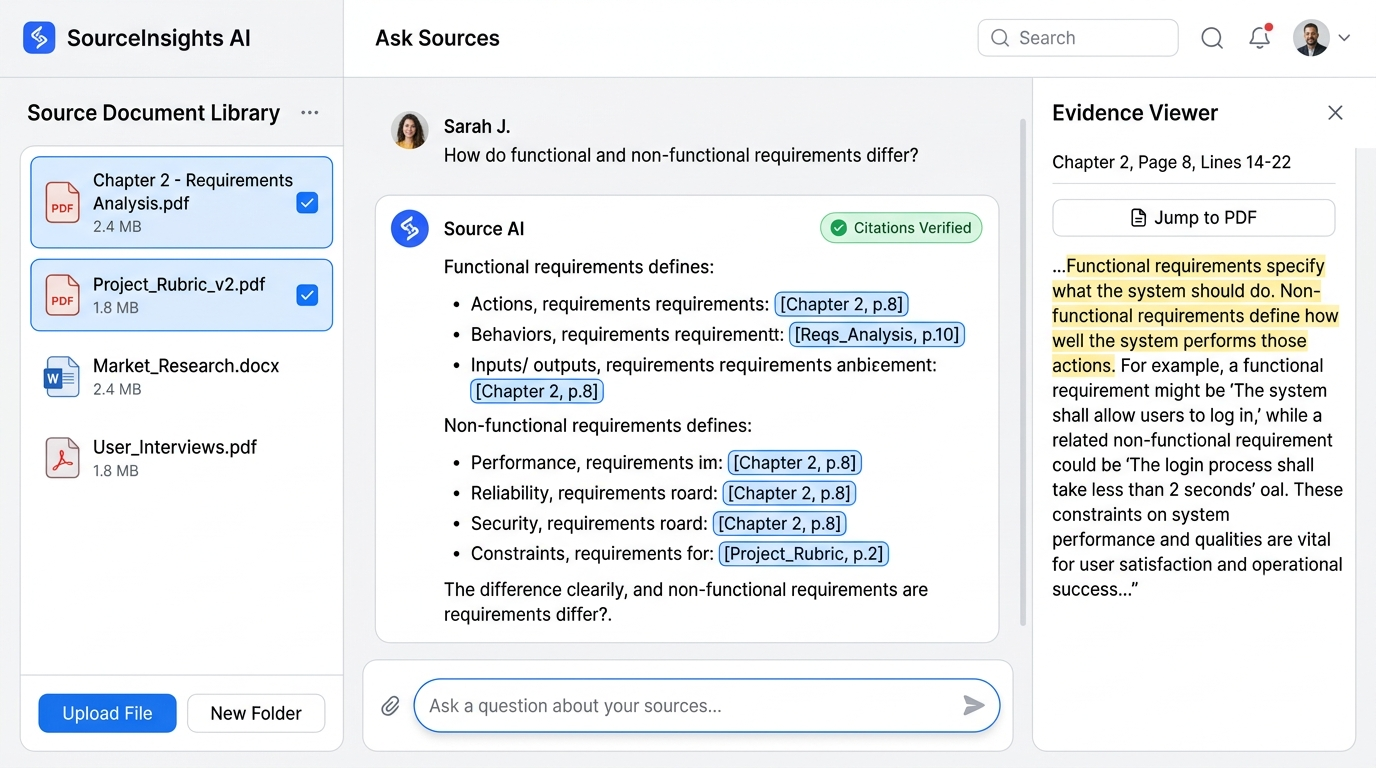
\includegraphics[width=0.88\linewidth,keepaspectratio]{img/chapter2/feature-1-4-en.png}

\caption{Feature 1 - User interface prototype for evidence-grounded Q\&A.}

\label{fig:feature-1-4}

\end{figure}



\needspace{3\baselineskip}

\paragraph*{Feature 2 Workflow: Document-Driven Progress Management}

The user requests task extraction from uploaded rubrics. Candidate requirements and tasks are reviewed in a confirmation drawer before being committed to the official database. Users manage active tasks across To Do, In Progress, and Done Kanban columns, and execute pure Python reconciliation against reference dates to expose missing coverage, overdue tasks, and date discrepancies.



\begin{figure}[!htbp]

\centering

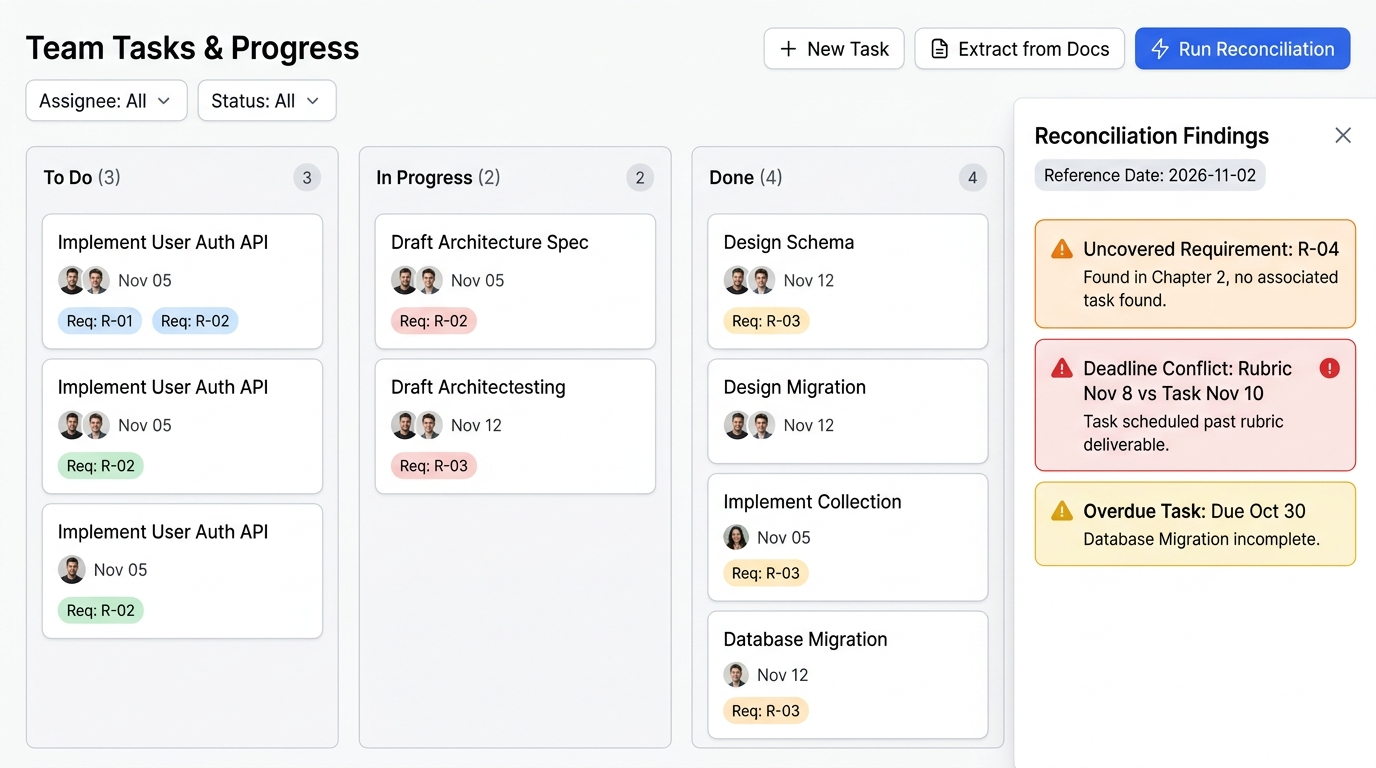
\includegraphics[width=0.88\linewidth,keepaspectratio]{img/chapter2/feature-2-4-en.png}

\caption{Feature 2 - User interface prototype for task board and progress management.}

\label{fig:feature-2-4}

\end{figure}



\needspace{3\baselineskip}

\paragraph*{Feature 3 Workflow: Context-Aware Email Reporting}

The user selects verified reconciliation findings to synthesize a progress email draft. After reviewing and modifying content, the user approves an exact snapshot, triggering SHA-256 payload hashing. Any post-approval edit revokes approval. Only when APPROVED, the user explicitly triggers dispatch, prompting the backend to submit the message via Gmail SMTP with STARTTLS.



\begin{figure}[!htbp]

\centering

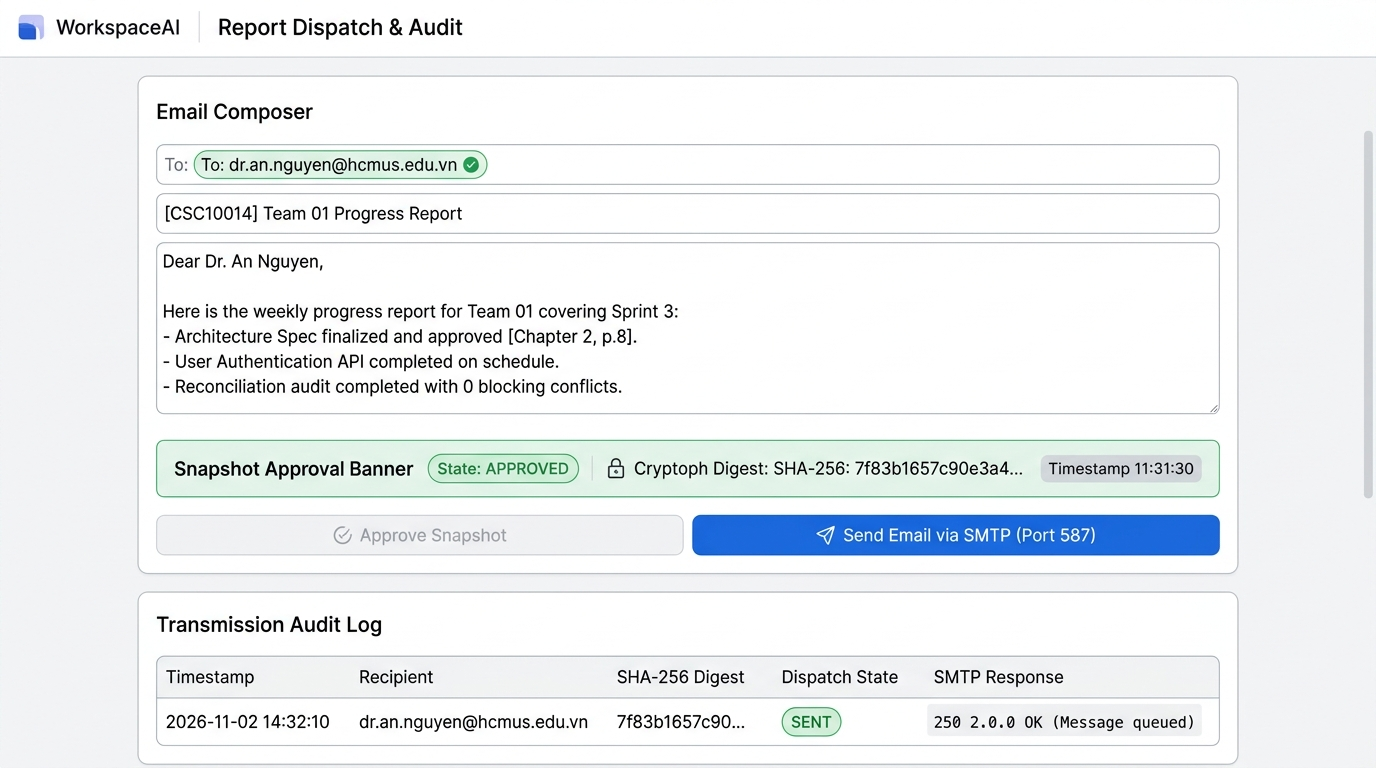
\includegraphics[width=0.88\linewidth,keepaspectratio]{img/chapter2/feature-3-4-en.png}

\caption{Feature 3 - User interface prototype for human-approved email reporting.}

\label{fig:feature-3-4}

\end{figure}



\FloatBarrier



% References cited in the synchronized Introduction.
\cleardoublepage
\phantomsection
\addcontentsline{toc}{chapter}{References}
\bibliographystyle{ieeetr}
\bibliography{ref/ref,ref/workspaceai}

% Appendix
% \appendix
% Add \cleardoublepage to move appendices to next page.
% \cleardoublepage
% \chapter{Các định lý}

\section{Một số định lý trong giải tích}

\subsection{Định lý giá trị trung bình}

\begin{theorem}[Định lý giá trị trung bình\cite{stewart12}]
Cho $f$ là một hàm liên tục trên khoảng đóng $[a, b]$ và khả vi trên khoảng mở $(a, b)$. Khi đó tồn tại một điểm $c \in (a, b)$ sao cho
$$
f'(c) = \frac{f(b) - f(a)}{b - a}
$$
\end{theorem}

\subsection{Định lý cơ bản của giải tích}

\begin{theorem}[Định lý cơ bản thứ I của giải tích\cite{stewart12}]
Cho $f$ là một hàm số thực liên tục trên khoảng đóng $[a, b]$. Gọi $F$ là hàm số xác định với mọi $x \in [a, b]$ sao cho
$$
F(x) = \int_a^x f(t)dt
$$
Khi đó $F$ liên tục trên $[a, b]$ và khả vi trên $(a, b)$, đồng thời với mọi $x \in (a, b)$, 
$$
F'(x) = f(x)
$$
vì thế $F$ là một \textbf{nguyên hàm} của $f$.
\end{theorem}

\begin{theorem}[Định lý cơ bản thứ II của giải tích\cite{stewart12}]
Cho $f$ là một hàm số thực trên khoảng đóng $[a, b]$ và $F$ là một hàm số liên tục trên $[a, b]$ và là một nguyên hàm của $f$:
$$
F'(x) = f(x)
$$
Nếu $f$ khả tích Riemann trên $[a, b]$ thì
$$
\int_b^a f(x)dx = F(b) - F(a)
$$
\end{theorem}
% \backmatter
\end{document}